\documentclass[12pt]{article}

% pacotes obrigatorios e formatacao
\usepackage[utf8]{inputenc}
\usepackage[T1]{fontenc}
\usepackage[brazil]{babel}
\usepackage[margin=2cm]{geometry} % margem minima de 2cm exigida pela metodologia
\usepackage{times} % fonte times new roman
\usepackage{graphicx}
\usepackage{booktabs}
\usepackage{xcolor}
\usepackage{listings}
\usepackage{fancyhdr}
\usepackage{hyperref}

% ---------------
% Resultados da enumeração. Use o comando abaixo para inserir screenshots:
% \begin{figure}[h!]
%     \centering
%     \includegraphics[width=0.8\textwidth]{screenshot_nmap.png}
%     \caption{Legenda descritiva da imagem inserida imediatamente após o texto.}
% \end{figure}

% \begin{lstlisting}[caption={Comando de exploração utilizado}]
% # Exemplo de bloco de código com fundo destacado
% nmap -sV -sC -oN scan.txt 10.10.10.10
% \end{lstlisting}
% ---------------

\definecolor{citapurple}{HTML}{6A1B9A} % tom roxo escuro
% configuracao de links (hierarquia e cores)
\hypersetup{
    colorlinks=true,
    linkcolor=black,       % cor para sumario, figuras (\ref) e secoes
    urlcolor=blue,         % cor para links de internet (\url, \href)
    citecolor=citapurple,  % cor para citacoes bibliograficas (\cite) em roxo
    pdftitle={WriteUp - CTF},
}

% configuracao dos blocos de codigo (monoespacado com fundo destacado)
\definecolor{codebg}{gray}{0.95}
\lstset{
    backgroundcolor=\color{codebg},
    basicstyle=\ttfamily\small,
    breaklines=true,
    frame=single,
    frameround=tttt,
    framesep=5pt,
    rulecolor=\color{gray!30},
    showstringspaces=false,
    keywordstyle=\color{blue},
    captionpos=b,
    inputencoding=utf8,
    extendedchars=true
}

% configuracao de cabecalho e rodape
\pagestyle{fancy}
\fancyhf{}
\lhead{\small \textit{Nome da Maquina - Plataforma}}
\rhead{\small \textit{Autor: nome (nickname)}}
\rfoot{\thepage} % numeracao de paginas obrigatoria

\begin{document}

% 2.1. capa
\begin{titlepage}
    \centering
    \vspace*{2cm}
    
    {\Huge \textbf{Nome da Máquina: Write Up}}\\[0.5cm]
    {\large \textbf{Plataforma:} HackTheBox}\\[1.5cm]
    
    \vfill
    
    % espaco dedicado para logotipo (plataforma, unbreakable ou da máquina)
    \begin{figure}[h!]
        \centering
        % substitua 'example-image' pelo arquivo da logo na pasta do projeto
        
\includegraphics[width=0.32\textwidth]{unbreakableLogo_3.png} 
    \end{figure}
    
    \vfill
    
    \begin{table}[h!]
        \centering
        \small
        \renewcommand{\arraystretch}{1.3}
        \begin{tabular}{ll}
            \textbf{Máquina / Desafio:} & Touch \\
            \textbf{Dificuldade:}       & Fácil \\
            \textbf{Autor:}             & Lurian Lima (luricl) \\
            \textbf{Matrícula:}         & 222005395 \\
        \end{tabular}
    \end{table}
    
    \vspace*{1.5cm}
    {\large \today}
\end{titlepage}

\newpage

% 2.2. sumario
% indice gerado automaticamente com numeracao de paginas
\tableofcontents
\newpage

% 2.3. visao geral
% paragrafo descrevendo o vetor principal de ataque sem spoiler detalhado.
% deve responder: o que e o desafio, qual a superficie explorada e o caminho geral ate o objetivo.
\section{Visão Geral}


% 2.4. reconhecimento
% resultados da enumeracao externa: portas abertas, servicos e versoes relevantes identificadas.
% incluir comandos executados em blocos de codigo e outputs truncados pertinentes.
% regra: nao incluir informacoes obtidas apos o foothold inicial.
\section{Reconhecimento}

Inicialmente, foi feita um reconhecimento usando o Nmap. Foi necessário adicionar a flag -Pn para evitar que o Nmap seja barrado pelo firewall ao tentar checar se há conexão. Com a flag, o Nmap parte direto para o scan.

\begin{lstlisting}[caption={Varredura de portas com Nmap}, label={lst:nmap}]
$ nmap -sV -T4 -Pn <TARGET_IP>
Starting Nmap 7.992 ( https://nmap.org ) at 2026-10-18 17:28 -0300
Nmap scan report for <TARGET_IP> (<TARGET_IP>)
Host is up (0.13s latency).
Not shown: 996 filtered tcp ports (no-response)
PORT     STATE SERVICE       VERSION
135/tcp  open  msrpc         Microsoft Windows RPC
3389/tcp open  ms-wbt-server Microsoft Terminal Service
5985/tcp open  http          Microsoft HTTPAPI httpd 2.0 (SSDP/UPnP)
8443/tcp open  http          Microsoft HTTPAPI httpd 2.0 (SSDP/UPnP)
Service Info: OS: Windows; CPE: cpe:/o:microsoft:windows

Service detection performed. Please report any incorrect results at https://nmap.org/submit/ .
Nmap done: 1 IP address (1 host up) scanned in 21.81 seconds
\end{lstlisting}

Como resultados, percebemos que o alvo é um host Windows (indicado pela linha \texttt{Service Info}), com quatro portas TCP abertas e 996 portas filtradas, ou seja, que não respondem. Essa proporção indica que um firewall descarta a maior parte do tráfego e deixa passar apenas alguns serviços, o que restringe a superfície de ataque a eles:

\begin{itemize}
    \item \textbf{135/tcp (MSRPC):} \textit{endpoint mapper} do RPC, usado por serviços do Windows para se registrarem e serem localizados. Pode ser enumerado depois para listar interfaces RPC, mas não dá acesso por si só.
    \item \textbf{3389/tcp (RDP):} Remote Desktop Protocol. Exige credenciais válidas, portanto só é útil após a obtenção de um usuário e senha.
    \item \textbf{5985/tcp (WinRM):} Windows Remote Management sobre HTTP, que permite executar comandos PowerShell remotamente. Também exige credenciais, mas é um dos caminhos mais diretos de acesso quando se possui uma conta válida.
    \item \textbf{8443/tcp (HTTP):} serviço web executado pelo \texttt{Microsoft HTTPAPI}. É a única porta com uma aplicação web aparente, e por isso é o ponto de partida natural para a análise.
\end{itemize}

Duas observações sobre a saída merecem atenção. Primeiro, a etiqueta \texttt{(SSDP/UPnP)} nas portas 5985 e 8443 não descreve o serviço real: o Nmap a atribui por correspondência de assinatura com o \texttt{HTTPAPI}, o servidor HTTP nativo do Windows, e não há indício de UPnP no alvo. Segundo, a porta 8443 foi identificada como HTTP e não como HTTPS, o que precisa ser confirmado manualmente, pois portas dessa família costumam usar TLS.

A porta 445 (SMB), comum em hosts Windows, não aparece entre as abertas. Como as portas não listadas são todas filtradas, ela não pode ser usada diretamente a partir desta varredura. Os próximos passos são verificar a aplicação na porta 8443 e confirmar o estado da porta 445. 

Podemos verificar se a porta 445 está aberta usando o nmap novamente.

\begin{lstlisting}[caption={Verificando o estado da porta 445 com Nmap}, label={lst:nmap-445}]
$ nmap -Pn -p 445 --reason <TARGET-IP>
Starting Nmap 7.992 ( https://nmap.org ) at 2026-10-18 17:48 -0300
Nmap scan report for <TARGET-IP> (<TARGET-IP>)
Host is up, received user-set.

PORT    STATE    SERVICE      REASON
445/tcp filtered microsoft-ds no-response

Nmap done: 1 IP address (1 host up) scanned in 2.02 seconds
\end{lstlisting}

Esse resultado indica que não houve resposta. Possivelmente, há um firewall descartando as respostas.

Porém, ao acessar o gobuster no link \textit{http://<TARGET-IP>:8443/}, descobrimos alguns diretórios:

\begin{lstlisting}[caption={Verificando diretórios com gobuster}, label={lst:gobuster-8443}]
$  gobuster dir -u http://<TARGET-IP>:8443/ -w /snap/seclists/current/Discovery/Web-Content/common.txt -t 50 -s 200,204,301,307,401,403 -b "" -o gobuster_8443.txt
..
/api                  (Status: 403) [Size: 35]
/favicon.ico          (Status: 200) [Size: 452]
/login                (Status: 200) [Size: 3572]
Progress: 4750 / 4750 (100.00%)
...
\end{lstlisting}

E, ao acessar o \textit{/login}, encontramos a seguinte tela:

\begin{figure}[h!]
    \centering
    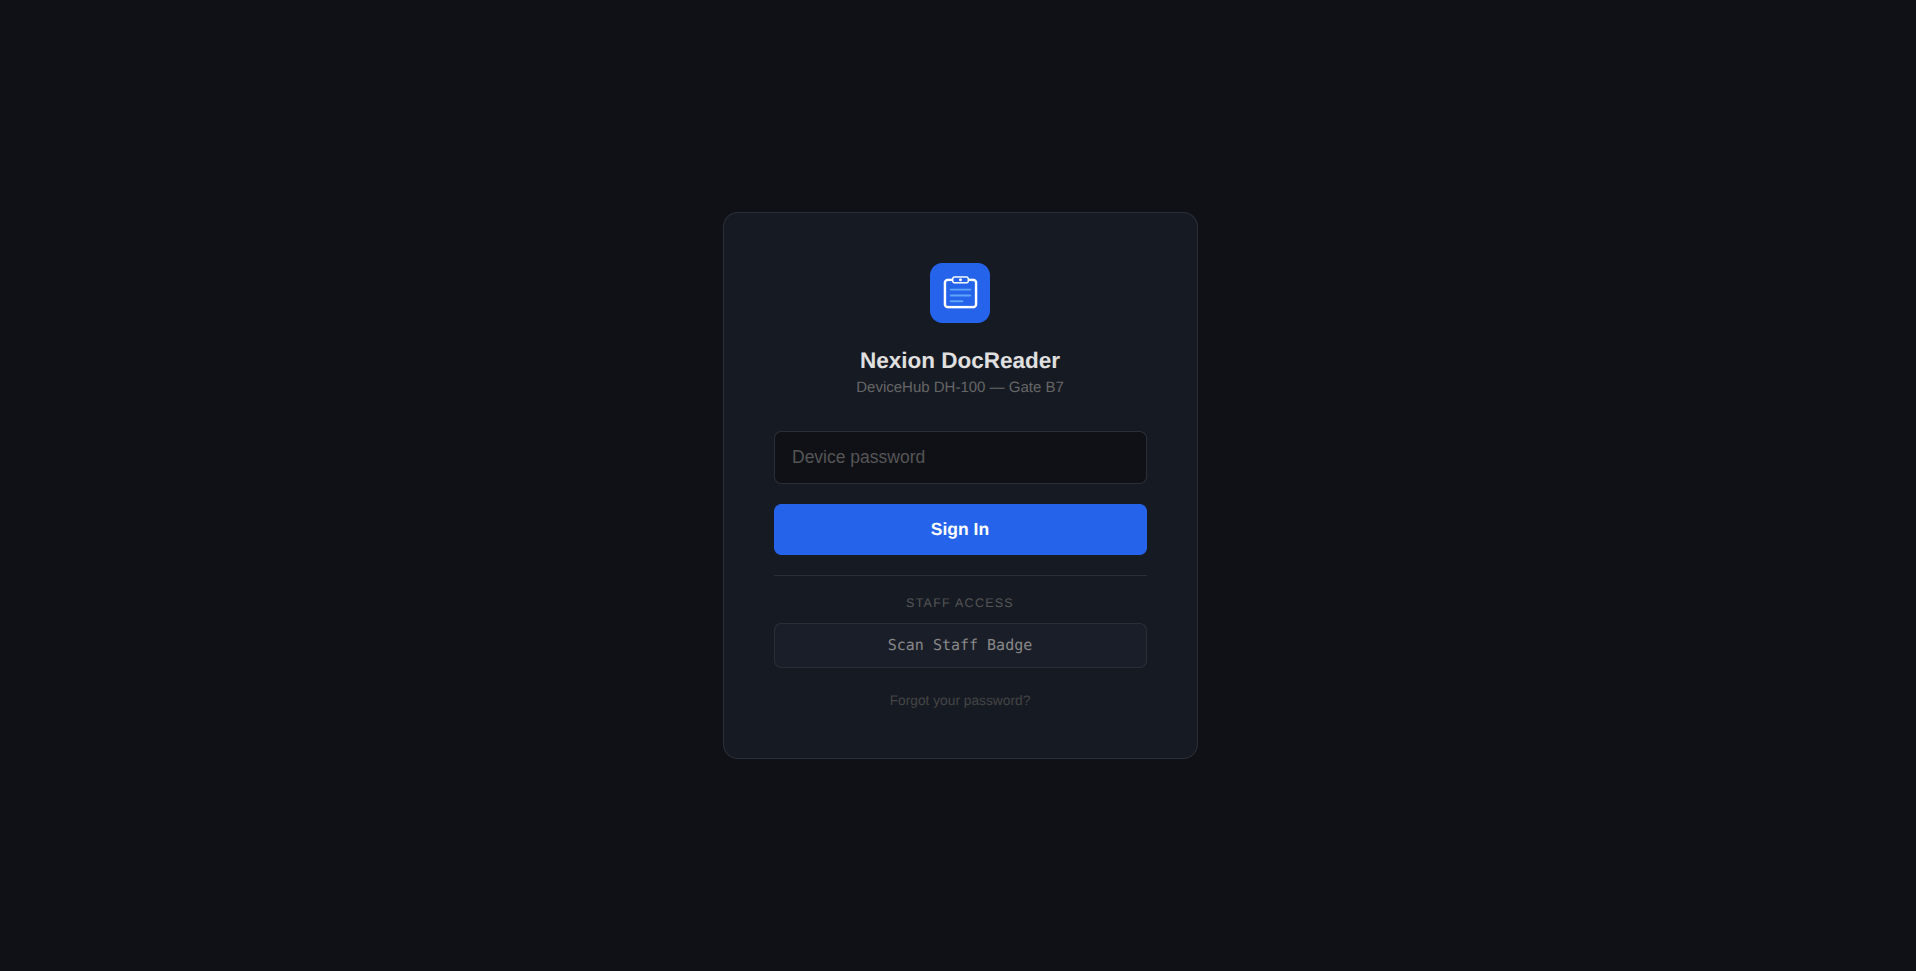
\includegraphics[width=0.45\textwidth]{imgs/tela_login.png}
    \caption{Tela encontrada.}
    \label{fig:tela_login}
\end{figure}

% 2.5. exploracao
% descricao tecnica detalhada do vetor de entrada e raciocinio que levou a vulnerabilidade.
% incluir scripts, exploits ou payloads utilizados (comentados) e justificativa dos passos.
% prints obrigatorios evidenciando o acesso inicial obtido (com placeholder para dados sensiveis).
\section{Exploração}

Examinando o html da página, é possível encontrar uma dica para a senha:

\begin{figure}[h!]
    \centering
    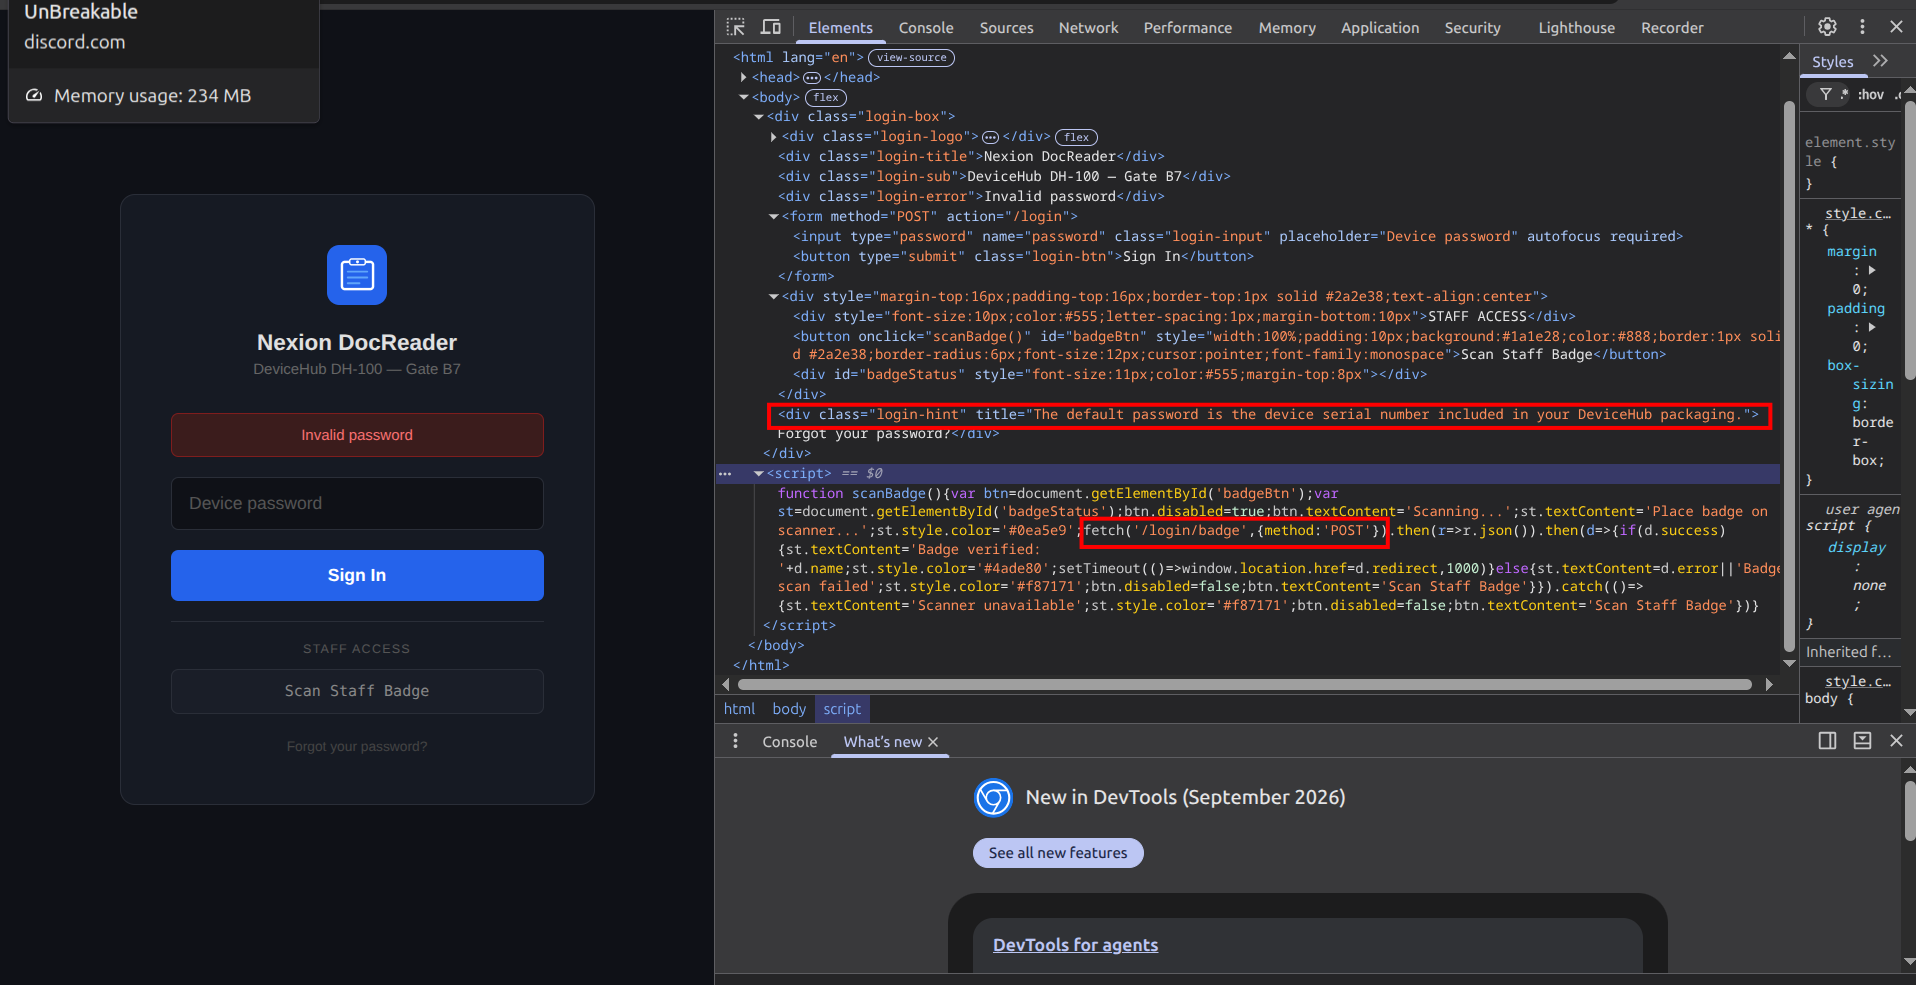
\includegraphics[width=0.45\textwidth]{imgs/html_pagina.png}
    \caption{Pistas encontradas no html da tela de login.}
    \label{fig:pistas_login}
\end{figure}

Como a dica da senha diz que a senha padrão é o número de série que vem na embalagem do dispositivo. Como não temos a embalagem, o caminho realista é procurar o número de série em algum lugar que o próprio alvo exponha.

Portanto, podemos explorar a rota \textit{/api}, que retorna o seguinte resultado:

\begin{lstlisting}[caption={Resultado obtido ao acessar a rota \textit{/api}}, label={lst:api-route}]
{"error":"Authentication required"}
\end{lstlisting}

Porém, o nome da rota sugere que podem haver outras rotas a partir dela, como \textit{/api/status/}, \textit{/api/info} ou \textit{/api/device} que devem entregar informações acerca do dispositivo. Ao acessar \textit{/api/status/}, encontramos as informações procuradas:

\begin{lstlisting}[caption={Informações obtidas ao acessar a rota \textit{/api/status}}, label={lst:api-status-route}]
{"device":"Nexion DeviceHub DH-100","serial":"NX-DH-2024-B7042","firmware":"1.4.2","status":"online","uptime":20774}
\end{lstlisting}

Logo, encontramos o número serial do dispositivo, que também é a senha, e somos redirecionados para a seguinte tela home:

\begin{figure}[h!]
    \centering
    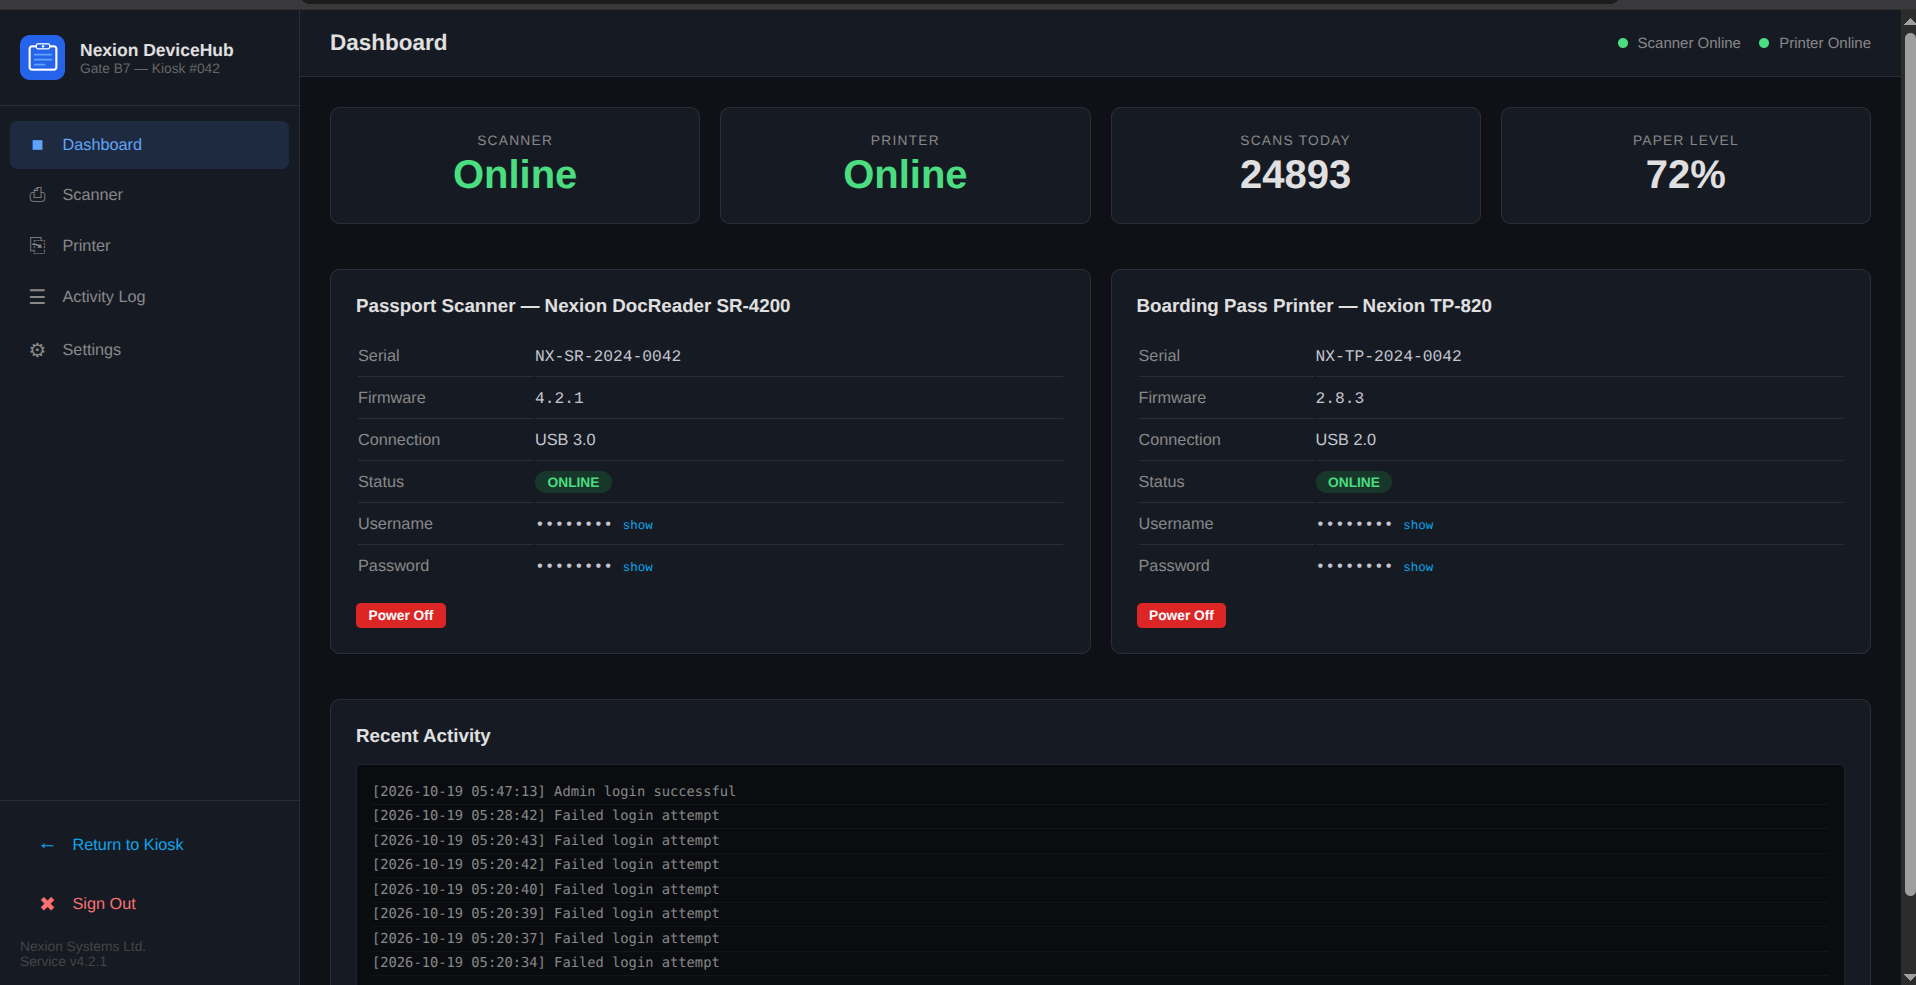
\includegraphics[width=0.45\textwidth]{imgs/tela_home.png}
    \caption{Tela home encontrada após o login.}
    \label{fig:tela_home}
\end{figure}

Nessa mesma tela, encontramos o Username e Senha de um usuário. Navegando para a aba \textit{scanner}, encontramos as mesmas credenciais:

\begin{figure}[h!]
    \centering
    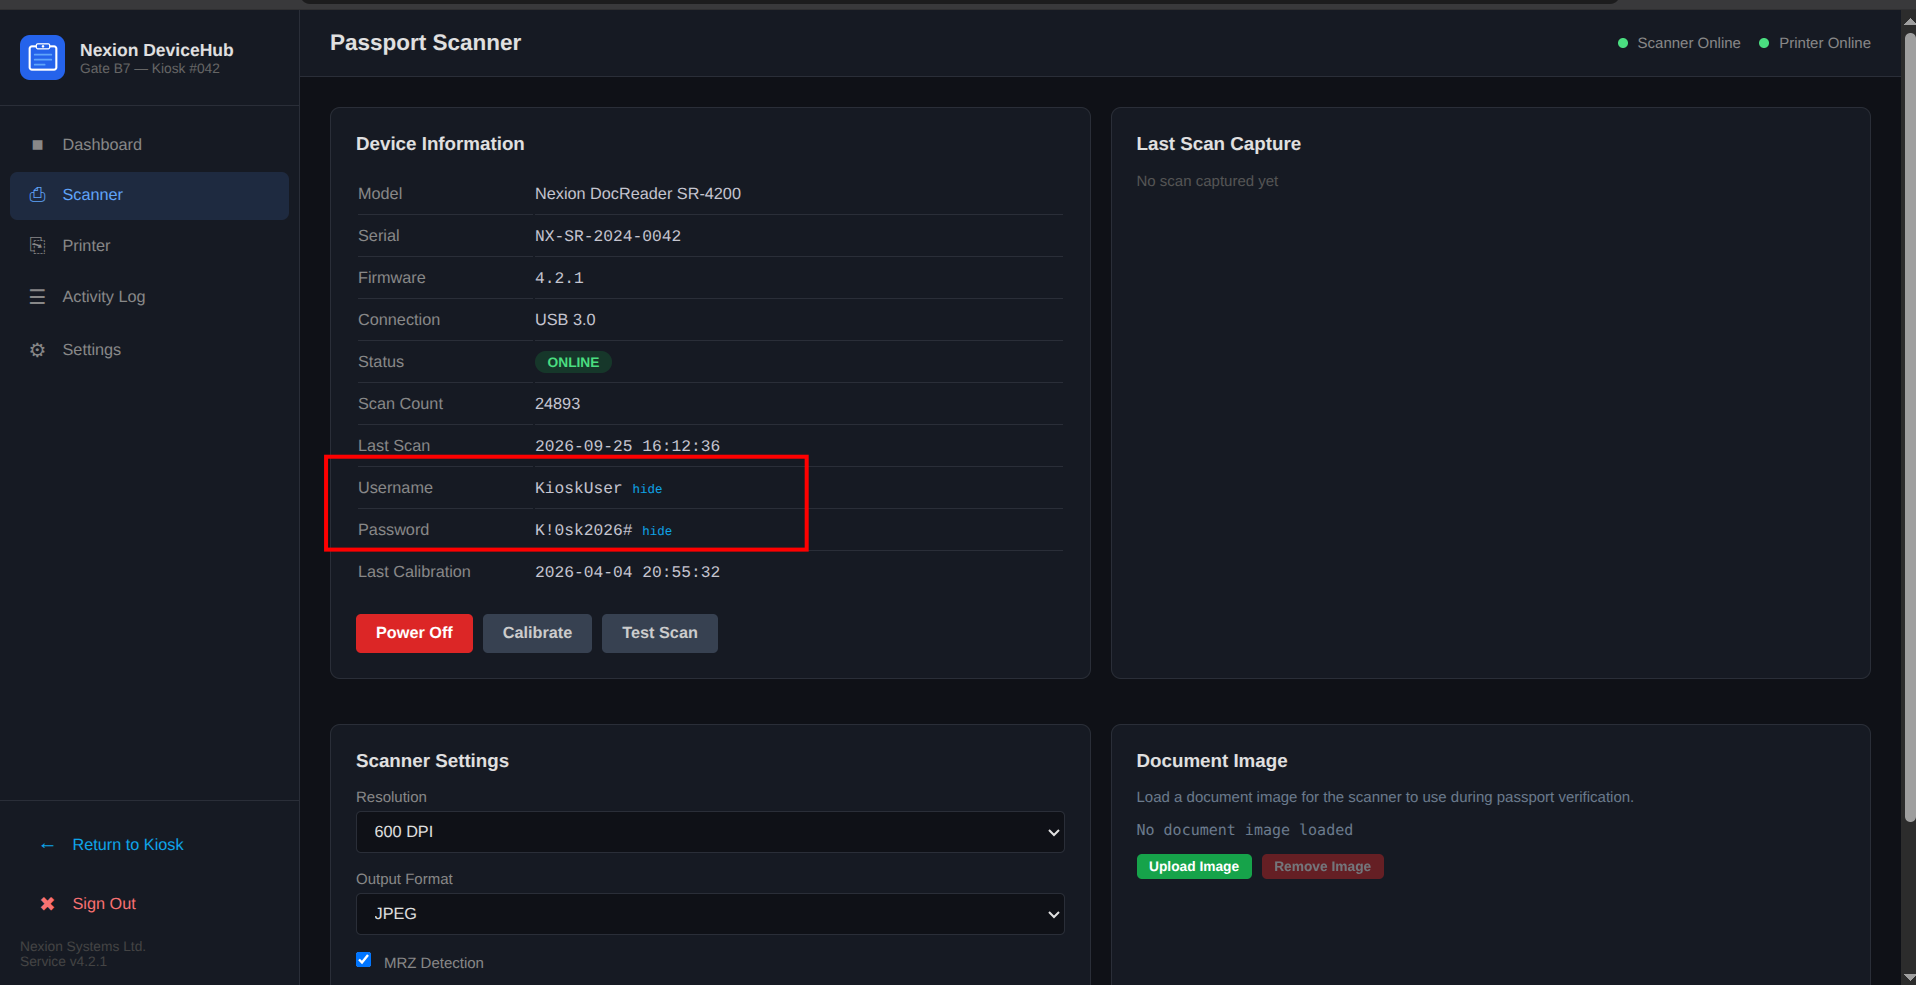
\includegraphics[width=0.45\textwidth]{imgs/user_pass_tela_scanner.png}
    \caption{Informações encontradas na tela scanner.}
    \label{fig:infos_tela_scanner}
\end{figure}

% 2.6. movimentacao lateral (se aplicavel)
% aplicavel quando ha multiplos usuarios no sistema ou necessidade de pivoting entre servicos.
% detalhar a escalada horizontal com comandos, raciocinio e evidencias necessarias.
\section{Movimentação Lateral}


% 2.7. escalada de privilegios
% descrever o vetor de privesc vertical, o processo de enumeracao local que o revelou
% (ex: linpeas, sudo -l, capabilities, binarios suid) e a exploracao realizada.
% incluir o comando final e captura que comprove o acesso root/system e as flags com placeholder.
\section{Escalada de Privilégios}


% 2.8. conclusao
% resumo tecnico de 3 a 5 linhas sintetizando a cadeia de exploracao completa,
% do reconhecimento a captura final da flag.
\section{Conclusão}

\section{Referências}

% 2.9. referencias
% espaco destinado as fontes utilizadas para a exploracao:
% links dos repositorios de exploits publicos, documentacoes e cves correspondentes.
\begin{thebibliography}{9}
    \bibitem{ref1}
    \textbf{OWASP / CVE / Nome da Vulnerabilidade}: Breve descrição técnica do vetor abordado, documentação ou payload de referência. \\
    Disponível em: \url{https://exemplo.com/artigo-ou-documentacao}
    
    \bibitem{ref2}
    \textbf{Repositório / Autor do Exploit}: Detalhes do exploit público, script ou ferramenta utilizada durante a exploração. \\
    Disponível em: \url{https://github.com/exemplo/repositorio-exploit}

\end{thebibliography}

\end{document}